% !TEX root = ../main.tex
\chapter{Le Web sémantique}
\label{annexe:semantic-web}

L'expression \emph{``Web sémantique''} trouve ces origines dans un
article révolutionnaire publié par Tim Berners-Lee \emph{et
  al.}~\cite{berners2001semantic} en \date{2001}. Le terme fait
d'abord référence à la vision du Web de demain comme un vaste espace
d'échange de ressources entre les êtres humains et les machines
permettant une exploitation, qualitativement supérieure, de grands
volumes d'informations et de services variés. D'après ses promoteurs
\emph{``le Web sémantique est une extension du Web actuel avec une
  signification bien définie des informations. Il permet une meilleur
  coopération et d'échanger l'information entre les ordinateurs et les
  utilisateurs.''}\medskip

Aujourd'hui, le Web Sémantique désigne une infrastructure
technologique visant à rendre le contenu des ressources du Web
accessible et utilisable par des logiciels ou des agents grâce à un
ensemble des langages et des standards initiés et maintenus par le
consortium \acrshort{w3c}. Ces langages sont organisés en couches
d'expressivité croissante permettant l'ajout d'une
\emph{\textbf{``sémantique explicite''}} au contenu des ressources
Web. Cette vision va transforme le Web actuel de documents en Web des
connaissances (ou \emph{Knowledgeable web}~\cite{decker2000semantic}),
ce qui contribue largement au développement de nouvelles approches
plus flexibles pour le partage des données, la réutilisation et
l'intégration de différentes applications.\medskip

%% TODO: éliminer la duplication du terme "Web sémantique"
Dans la suite, nous introduisons la vision globale du Web sémantique,
leur objectifs et principes
fondamentaux~\ref{sec:semantic-web-vision}. Ensuite Nous allons
présenter les principaux standards et langages développés par la
communauté pour la réalisation et la concrétisation du web
sémantique~(\ref{sec:semantic-web-rdf}~\ref{sec:semantic-web-owl2}).

\newpage
\section{La vision du Web sémantique}
\label{sec:semantic-web-vision}

%!TEX root = ../../main.tex
\begin{figure}[h]
    \centering
    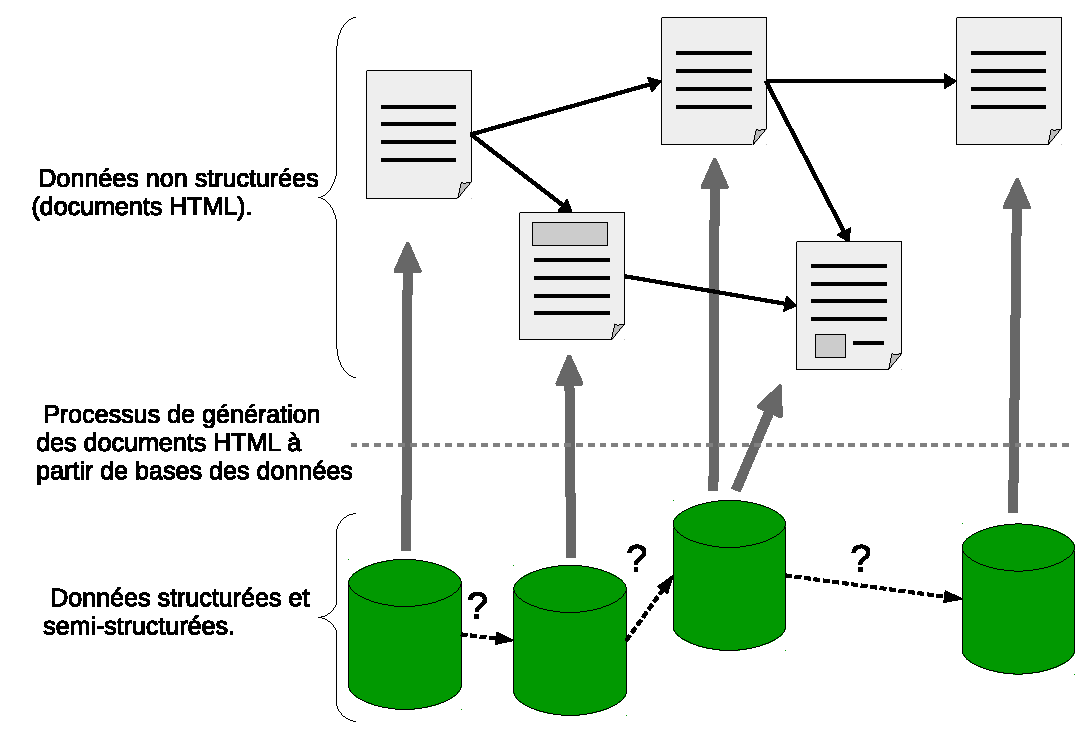
\includegraphics[width=1\textwidth]{figs/A/structured-and-unstructured-data-on-the-web.eps}
    \caption{Les données structurés et non-structurés du
      Web~\cite{antoniou2012semantic}.}\label{fig:structured-and-unstructured-data-on-the-web}
\end{figure}
%%% Local Variables:
%%% mode: latex
%%% TeX-master: "../../main"
%%% End:


% des phrases trop longues !!
Le Web actuel est essentiellement \emph{\textbf{syntaxique}}, dans le
sens que la structure des documents est bien définie mais que son
contenu reste quasi inaccessible aux traitements machines. Il s'agit
d'un Web de documents, les ressources sont structurées en
\acrshort{html} et identifiés de manière unique par des \acrshort{uri}
reliés entre eux par des liens \emph{hypertextes}. L'information est
essentiellement textuelle et la structure riche qui est généralement
conçus au préalable dans des schémas relationnelles est presque
complètement perdu dans le processus de publication de telles données
sous formes des documents \acrshort{html} (ce qui illustré dans la
figure~\ref{fig:structured-and-unstructured-data-on-the-web}).\medskip

La nouvelle génération de Web nommée \emph{``Le Web sémantique''} a
pour ambition de lever cette difficulté. Les ressources du Web seront
plus aisément accessibles aussi bien par l'homme que par la machine,
grâce à la représentation \emph{\textbf{sémantique}} de leurs
contenus. La suite de cette section a pour but de expliquer les
principes fondamentaux et les idées principales derrière le Web
sémantique~\ref{sec:semantic-web-design-decisions}, ainsi que le socle
technologique permettant la concrétisation de ces
idées~\ref{sec:semantic-web-stack}.\medskip

\subsection{Principes fondamentaux du Web sémantique}
\label{sec:semantic-web-design-decisions}

Le Web sémantique, ou le Web de données (dans son vision
futuriste~\cite{bizer2008linked}) suit différents principes de
conception, qui peuvent être résumés comme
suit~\cite{antoniou2012semantic}:\medskip

\begin{enumerate}
\item Rendre les données structurées et semi-structurées (illustré
  dans la
  figure~\ref{fig:structured-and-unstructured-data-on-the-web})
  disponibles dans formats normalisés et standardisés sur le
  Web;\medskip

\item Rendre non seulement les ensembles de données, mais aussi les
  éléments individuels de données et leurs relations implicites
  accessibles sur le Web;\medskip

\item Décrire la sémantique de ces données dans un formalisme bien
  définie, afin que cette sémantique peuvent être accessibles et
  traitables par des machines.
\end{enumerate}

Ces décisions conceptuelles sont la résultat directe d'un aperçu
principal qui nous amène à un grand progrès vers la vision du Web
sémantique. En effet, l'idée générale est de publier et interconnecter
l'structure sous-jacente de l'ensemble de données au lieu de
simplement publier et interconnecter des pages
\acrshort{html}.\medskip

Un aspect clé du Web est le fait que son contenu est totalement
distribué~\cite{berners1989information}, cette caractéristique
fondamentale contribue énormément à la naissance et la propagation de
Web tel que nous le connaissons aujourd'hui. En effet, la vision du
Web sémantique doit prendre en compte de la nécessaire ouverture du
Web et son architecture décentralisée, cette rétrocompatibilité
manifeste dans la traduction des trois principes mentionnées
précédemment sous forme d'un ensemble de décisions techniques
~\cite{antoniou2012semantic}:\medskip

\begin{enumerate}
\item Utiliser un graphe étiqueté comme un modèle de données pour
  représenter les ressources Web et ses relations. Le standard
  \acrshort{rdf} (parfois nommé un langage) est utilisé comme un
  formalisme pour représenter ces graphes;\medskip

\item Utiliser \acrshort{uri} pur identifier les éléments de données
  individuels et ses relations qui apparaissent dans la structure de
  données sous-jacente. Encore une fois, cela se reflète dans la
  conception du \acrshort{rdf}.;\medskip

\item Utiliser des ontologies (vocabulaires hiérarchiques de types et
  de relations) pour représenter formellement la sémantique prévues
  des données. Des formalismes tels que \acrshort{rdfs} et
  \acrshort{owl} sont utilisés pour ce effet.
\end{enumerate}\bigskip

\newpage
\subsection{Technologies clés du Web sémantique}
\label{sec:semantic-web-stack}

Pour la mise en place d'un Web sémantique, un ensemble des étapes
doivent être considérées pour l'implémentation des principes
ci-dessus~\ref{sec:semantic-web-design-decisions}. Premièrement, il
faut un \textbf{syntaxe standard} pour représenter les données et les
\emph{méta-données}. Deuxièmement, Avoir un accord suffisant sur un
\textbf{vocabulaire} pour les \emph{méta-données} afin de partager la
sémantique prévues des données. Enfin, publier un grand volume de
données dans les formats de la première étape en utilisant les
vocabulaires de la deuxième étape~\cite{antoniou2012semantic}.\medskip

%!TEX root = ../../main.tex
\begin{figure}[h]
    \centering
    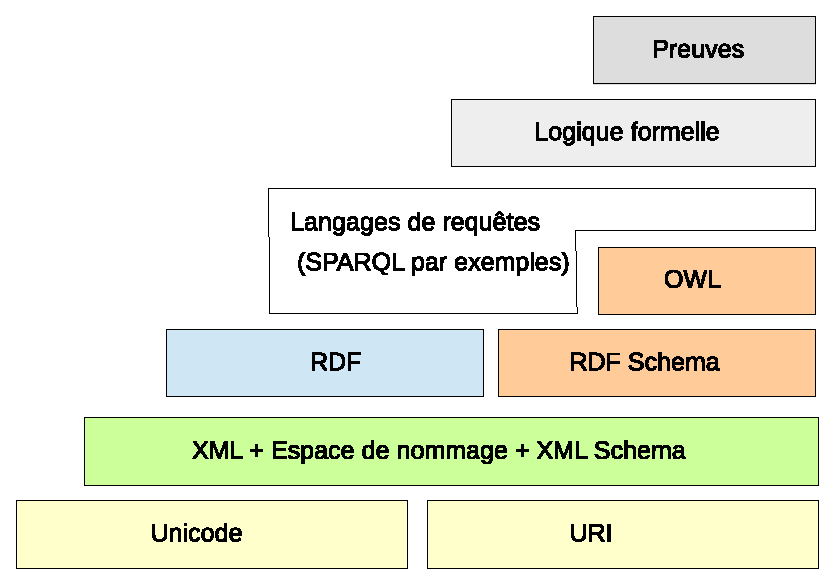
\includegraphics[width=0.85\textwidth]{figs/A/semantic-web-stack.eps}
    \caption{La pyramide du Web sémantique.}\label{fig:semantic-web-stack}
\end{figure}
%%% Local Variables:
%%% mode: latex
%%% TeX-master: "../../main"
%%% End:


Au cours de les deux dernières décennies, des progrès substantiels ont
été réalisés dans chacun de ces trois étapes. Des langages comme
\acrshort{rdf}, \acrshort{rdfs} et \acrshort{owl} (organisés en
couches d'expressivité croissante) ont reçu l'appui officiel du
consortium \acrshort{w3c}. Cet ensemble de \emph{``couches''} est
appelé, par ce dernière, \emph{``la pyramide des langages du Web
  sémantique''} (illustrée dans la
figure~\ref{fig:semantic-web-stack}). Plusieurs milliers de
vocabulaires ont été publiés dans ces formats (vocabulaire
schema.org~\footnote{\url{http://schema.org/}}, par exemple), ainsi
que le développement rapide du \emph{Linked
  Data}~\footnote{\url{http://linkeddata.org/}} a donné lieu à de
nombreux milliards d'objets et leurs relations deviennent disponibles
sur le Web s'appuyant sur une syntaxe et des vocabulaires communes.

Deux types de bénéfices sont motivés par cette organisation en couches
des langages du Web sémantique illustrée dans
figure~\ref{fig:semantic-web-stack}:\medskip

\SpecialItem
\begin{itemize}
\item Elle doit permettre de choisir le langage d’expressivité et de
  complexité adapté aux besoins d'une modélisation à réaliser;\medskip

\item Elle permet une approche graduelle dans les processus de
  standardisation de ces langages naissants (\acrshort{owl} n'a vu
  le jour qu'en \date{2001}~\cite{fensel2001oil} et est une
  recommendation du \acrshort{w3c} depuis seulement
  \date{2004}~\cite{mcguinness2004owl}).\medskip
\end{itemize}
\enddescription

Dans la construction d'une couche du Web sémantique sur le dessus de
l'autre, deux principes doivent suivie~\cite{antoniou2012semantic}:

\renewcommand{\descriptionlabel}[1]{\hspace{0.5cm}\textbullet~\textsf{#1}}
\begin{description}
\item[Compatibilité descendante]: Les agents logiciels spécialisés
  d'une couche devraient également être en mesure d'utiliser et
  interpréter l'information écrite à des niveaux inférieurs de
  pyramide. Par exemple, les agents qui peuvent accéder à la
  sémantique de \acrshort{owl} peuvent profiter pleinement des
  informations exprimées en \acrshort{rdf} et \acrshort{rdfs};

\item[Compatibilité ascendante partielle ]: Les gents logiciels
  spécialisés d'une couche devrait être en mesure de profiter au moins
  \textsf{partiellement} de l'information aux niveaux plus élevés. Par
  exemple, un agent spécialisé seulement à l'analyse syntaxique des
  documents \acrshort{rdf} et \acrshort{rdfs} pourraient interpréter
  une connaissance exprimée en \acrshort{owl} partiellement.
\end{description}
\enddescription

La figure~\ref{fig:semantic-web-stack} montre \emph{``la pyramide du
  Web sémantique''} qui décrit les couches principales de la
conception du Web sémantique. Cette vision est proposée initialement
par Tim Berners-Lee~\cite{berners2000xml} en \date{2000} au sien de
\acrshort{w3c}.\medskip

Le bas de la pyramide correspond aux technologies rassemblées sous le
nom du web de documents et qui permettre de fournir les bases du Web
sémantique. Nous trouvons à dans ce niveau là, l'dentificateur de
ressource internationalisé~\acrshort{uri}~\footnote{Il faut bien noter
  la différence entre les spécifications URL, URL et URN expliquée
  dans ce lien \url{http://www.w3.org/TR/uri-clarification/}.} qui
permet d'attribuer un \emph{identifiant unique} à un ensemble de
ressources sur le Web (documents, numéros téléphone, numéros
\acrshort{isbn}, etc), ainsi que le standard
\textsf{Unicode}~\footnote{\url{http://unicode.org/}.}  pour le codage
de textes dans différentes langues.\medskip

\acrshort{xml}~\cite{bray1998extensible} est un composant fondamental
qui assure \emph{l'interopérabilité
  syntaxique}~\cite{decker2000semantic} de cette infrastructure, il
fournit un mécanisme simple et puissant pour représenter des données
échangeables sur le Web. Le langage
\acrshort{xmls}~\cite{fallside2004xml} permet de construire des
documents \acrshort{xml} suivant un syntaxe et une structure
hiérarchique spécifique et les étendre avec des types de
données.\medskip

\acrshort{rdf}~\cite{lassila1999resource} est le modèle de données
fondamental pour le Web sémantique, il permet d'une meilleure
représentation et exploitation des \emph{méta-données} structurées et
fournit un support pour \emph{l'interopérabilité
  sémantique}~\cite{decker2000semantic}. \acrshort{rdfs}~\cite{brickley2000resource}
est un langage qui sert á définir un vocabulaire pour décrire les
propriétés et les classes des ressources \acrshort{rdf} et fixer une
\emph{sémantique} partagée des ressources Web.\medskip

\acrshort{rdfs} peut être considéré comme un langage primitive pour la
représentation des connaissances et de définir des
ontologies~\cite{antoniou2012semantic}. \acrshort{owl}~\cite{martin2004owl}
ajoute plus de vocabulaire pour décrire les propriétés et les classes,
les relations entre les classes, cardinalité, égalité, typage de
propriétés plus riche, caractéristiques des propriétés et les
hiérarchies des propriétés et des classes.\medskip

Les couches supérieures de l'architecture de Web sémantique
contiennent la couche logique qui permet de l'écriture des règles
logiques de raisonnement et d'inférence et la couche de preuve qui
exécute et évalue ces règles utilisées.


\section{La description des ressources Web: RDF(S)}
\label{sec:semantic-web-rdf}

%TODO: vérifier surtout la dernière phrase entres les parenthèses.
\acrshort{rdf} fournit un modèle de données flexible et indépendant de
tout domaine pour représenter les données et \emph{méta-données}
sous-jacentes du Web~\cite{decker2000semantic}, son composant de base
est le triplet \emph{``suject-propriété-object''}, appelé une assertion
ou encore une déclaration (\emph{``Statement''} en Anglais), c'est
pourquoi il est mentionné parfois comme un langage assertionnel. Il
faut bien noter la standard \acrshort{rdf} n'exige aucun format
particulier pour la sérialisation (et que \acrshort{xml} est juste un
autre).\medskip

%% TODO: Why use RDF?

\newpage
Puisque le \acrshort{rdf} est pas lié à un domaine particulier, il est
nécessaire pour un utilisateur de définir \emph{une terminologie}
qu'ils utilisent au sein de ces déclarations. Le langage
\acrshort{rdfs} permet aux utilisateurs de définir précisément comment
leur vocabulaire (leur terminologie) doit être interprétée, c'est
l'habileté de attribuer une \emph{\textbf{sémantique explicite}} à un
ensemble de données (ressources Web).\medskip

Pour résumer, \acrshort{xml} peut être vu comme la couche de
sérialisation syntaxique, \acrshort{rdf} comme un modèle de
base. \acrshort{rdfs} offre des primitives de représentation de
connaissances structurées en \acrshort{rdf} et l'ajoute une sémantique
prévue.\medskip

Dans cette section, nous présentons le standard \acrshort{rdf}
~\ref{sec:semantic-web-rdf-rdf}, ainsi que ses syntaxes courantes pour
le sérialiser. Ensuite, Les bases de langage \acrshort{rdfs} et ses
composantes principales sont introduites
en~\ref{sec:semantic-web-rdf-rdf}.\medskip

\subsection{RDF~: Le modèle de données}
\label{sec:semantic-web-rdf-rdf}

les concepts fondamentaux de \acrshort{rdf} sont les ressources, les
propriétés, les assertions (déclaration) et les graphes.

\subsubsection{Ressources}
\label{sec:semantic-web-rdf-rdf-resources}

Une ressource est un élément constitutif de base de l'architecture du
Web, elle désigne un entité qui peut être référencé par une
\acrshort{uri}. Cela veut dire qu'une ressource peut être une page Web
mais pas nécessairement, il peut désigne également un élément non
présent physiquement sur le Web comme un livre imprimé, qui sera alors
référencé par exemple par son numéro \acrshort{isbn}.

\subsubsection{Propriétés}
\label{sec:semantic-web-rdf-rdf-properties}

Une propriété (ou une prédicat) est une ressource qui décrit une
relation binaire entres deux autres ressources, par exemple
\emph{``écrit par''} et \emph{``est de type de''}. Comme toutes les
ressources, les propriétés sont identifiées par des
\acrshort{uri}. Une propriété peut être aussi \emph{déréférencée} pour
accéder à sa description textuelle.

\subsubsection{Assertions}
\label{sec:semantic-web-rdf-rdf-statements}

La structure fondamentale en \acrshort{rdf} est un triplet $<S,P,O>$
composé d'un sujet $S$, une propriété $P$ et un objet $O$. Un triplet
s'interprète comme suit: \emph{``le sujet $S$ a pour propriété $P$
  l'objet $O$''}, Chaque composant du triplet est aussi appelé sous le
terme générique de ressource, mais est généralement utilisé pour
parler du sujet ou de l'objet~\cite{antoniou2012semantic}.\medskip

%!TEX root = ../../main.tex
\begin{figure}[h]
    \centering
    \begin{subfigure}[b]{1\textwidth}
    \centering
    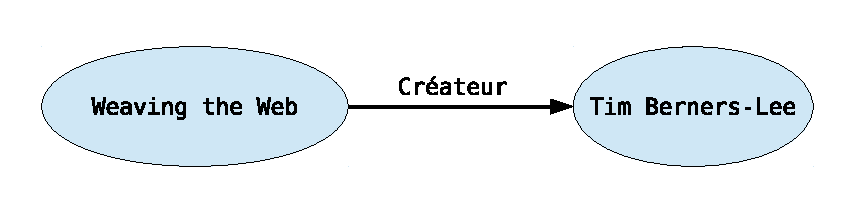
\includegraphics[width=0.85\textwidth]{figs/A/rdf-statement-example-graph.eps}
    \caption{Une illustaion graphique d'une assertion
      \acrshort{rdf}.}~\label{fig:rdf-statement-example-graph}
    \end{subfigure}

    \begin{subfigure}[b]{1\textwidth}
      \centering
      \lstinputlisting[language={XML}]{figs/A/rdf-statement-example.rdf}
      \caption{Une représentation \acrshort{rdf/xml} de l'assertion illustrée
        dans las
        figure~\ref{fig:rdf-statement-example-graph}.}~\label{fig:rdf-statement-example-rdf/xml}
    \end{subfigure}

    \caption{Un exemple d'une assertion
      \acrshort{rdf}.}~\label{fig:rdf-statement-example}
\end{figure}
%%% Local Variables:
%%% mode: latex
%%% TeX-master: "../../main"
%%% End:


%% TODO: dénote vs énoncer s vs exprimer
La figure~\ref{fig:rdf-statement-example-graph} représente un exemple
d'une une assertion \acrshort{rdf} qui dénote que l'auteur Tim
Berners-Lee est l'auteur du livre \emph{``Weaving the Web''}.\medskip

%% TODO: redondance, des mots répétés !!
le modéle \acrshort{rdf} décrit dans cette section est considéré comme
une syntaxe abstraite pour la représentation des données et
\emph{méta-données}. En effet, ce modèle est indépendant d'une toute
syntaxe concréte particulière, des différentes syntaxes concrètes
(comme \acrshort{rdf/xml}, celle qui est montrée dans la
figure~\ref{fig:rdf-statement-example-xml}) peuvent produire
exactement le même modèle du point de vue de sa syntaxe
abstraite.\medskip

\subsubsection{Graphes}
\label{sec:semantic-web-rdf-rdf-graphs}

La figure~\ref{fig:rdf-statement-example-graph} représente une
assertion \acrshort{rdf} sous forme d'un graphe orienté et
étiqueté. Les nœuds d'un tel graphe représentent les sujets ou les
objets, ils sont connectés par des arcs orienté à partir du sujet de
l'assertion à son objet, avec une étiquette sur l'arc représentant la
propriété de cette assertion.\medskip

La figure~\ref{fig:rdf-statement-example-xml} est supposé d'être la
concrétisation syntaxique du modèle abstrait dénoté par
l'assertion. Cependant, et pour des raisons de clarté et de
lisibilité, la figure~\ref{fig:rdf-statement-example-graph} n'illustre
qu'une seule assertion contenant dans le fichier \acrshort{rdf/xml} et
sans tenant compte des valeurs réelles identifiées par des
\acrshort{uri}.\medskip

%!TEX root = ../../main.tex
\begin{figure}[h]
    \centering
    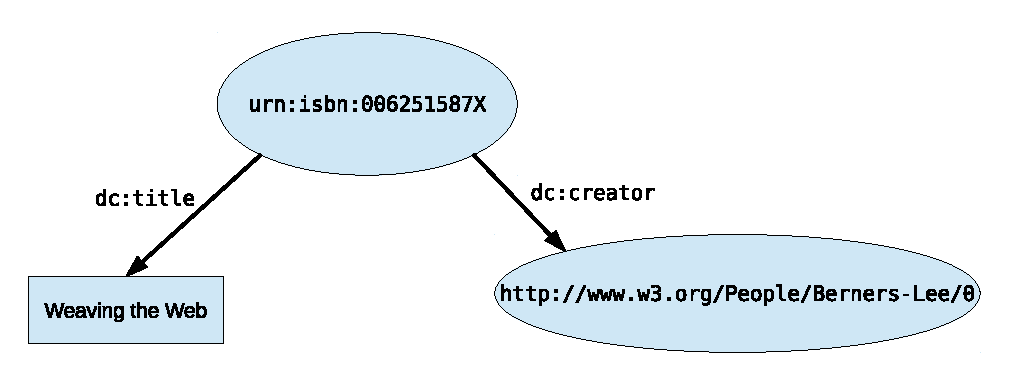
\includegraphics[width=1\textwidth]{figs/A/rdf-graph.eps}
    \caption{Un graphe qui représente un ensemble des assertions
      \acrshort{rdf}.}\label{fig:rdf-graph}
\end{figure}
%%% Local Variables:
%%% mode: latex
%%% TeX-master: "../../main"
%%% End:


Le graphe illustré dans la figure~\ref{fig:rdf-graph} reflète
exactement la structure exprimée en \acrshort{rdf/xml} dans l'exemple
précédant~\ref{fig:rdf-statement-example-xml}, il représente un modéle
constitué de deux assertions \acrshort{rdf} qui partage une ressource
commune (le même sujet).\medskip

Cette représentation graphique souligne l'idée que le standard
\acrshort{rdf} est essentiellement un modèle de graphe orienté et
étiqueté. Il est important aussi de noter que ce graphe est souvent
créé dans un environnement distribué (le Web) où plusieurs
participants peuvent partager et relier différentes ressources basant
sur la réutilisation des \acrshort{uri}. Cela nous amène au Web de
données qui nous permet de publier, exploiter et réutiliser des
données fortement connectées (\emph{``Smart
  Data~\cite{allemang2011semantic}''}) au lieu de publier des
documents soutenu par des structures de données globalement isolées
(\emph{``Dumb Data~\cite{allemang2011semantic}''}).\medskip

\subsection{RDFS~: L'ajout de sémantique}
\label{sec:semantic-web-rdfs}

\acrshort{rdfs}~\cite{brickley2000resource} est un langage destiné à
la représentation des connaissances, il a pour but d'étendre
\acrshort{rdf} en fournissant une structuration aux ressources
utilisées. \acrshort{rdfs} ajoute à \acrshort{rdf} des éléments de
bases dotés d'une sémantique fixée pour la définition de vocabulaires
d'un certain domaine applicatif.\medskip

Ce langage est une première étape pour modéliser des ontologies sur le
Web Sémantique~\cite{passant2009technologies}. Il introduit les
notions de classe (\texttt{rdfs:Class}) et de propriété
(\texttt{rdfs:Property}) associées à des relations de sous-classe
(\texttt{rdfs:subClassOf}) et de sous-propriétée
(\texttt{rdfs:subPropertyOf}). \acrshort{rdfs} permet également pour
chaque propriété de définir son domaine (\texttt{rdfs:domain}) et son
co-domaine (\texttt{rdfs:range}). La
figure~\ref{fig:rdfs-vs-rdf-layers} (la partie colorée en orange)
illustre graphiquement les relations qui existent entre les
différentes primitives du langage \acrshort{rdfs}.

%!TEX root = ../../main.tex
%!TEX root = ../../main.tex
\begin{figure}[h]
    \centering
    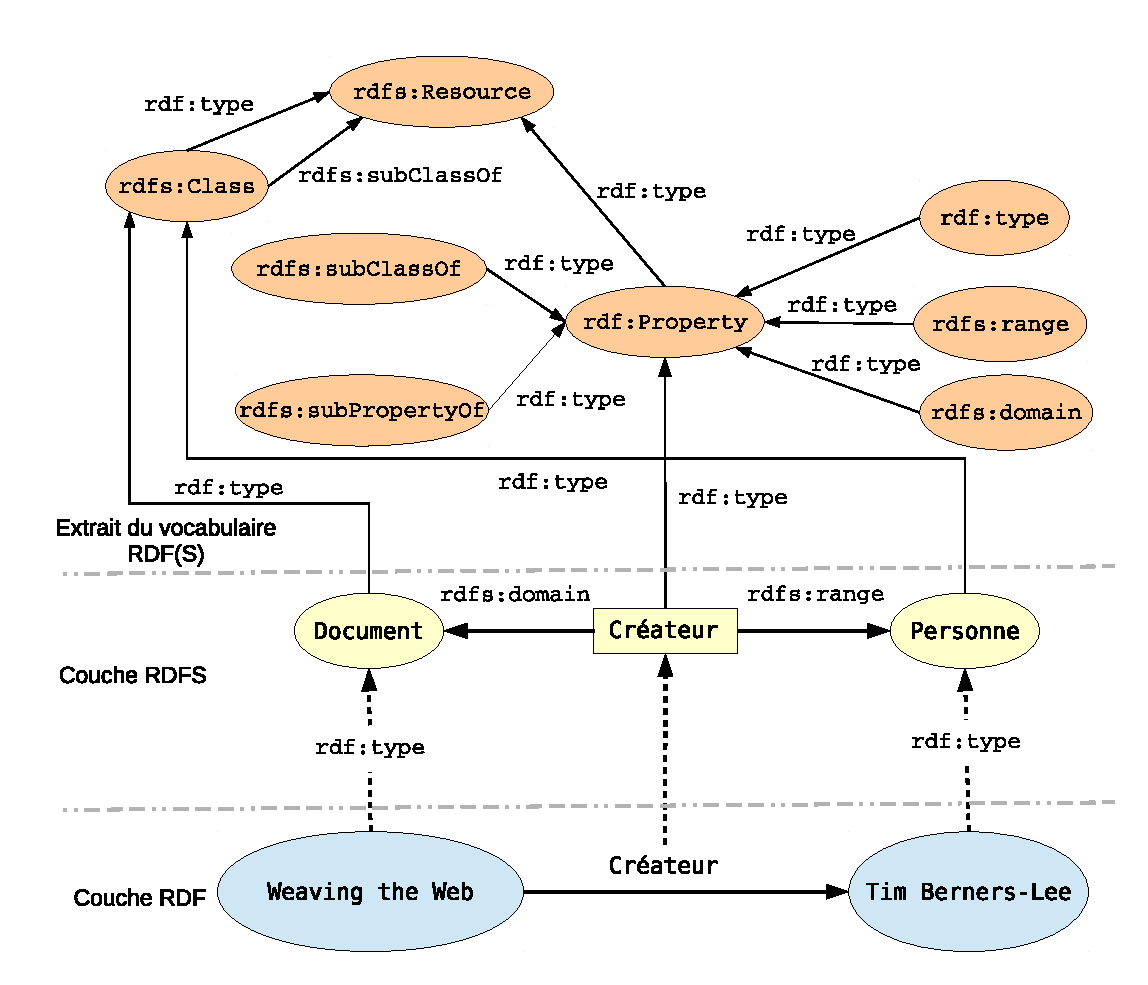
\includegraphics[width=1.05\textwidth]{figs/A/rdfs-vs-rdf-layers.eps}
    \caption{Les couches \acrshort{rdf} et \acrshort{rdfs} du Web
      sémantique.}\label{fig:rdfs-vs-rdf-layers}
\end{figure}
%%% Local Variables:
%%% mode: latex
%%% TeX-master: "../../main"
%%% End:


L'exemple illustré dans la figure~\ref{fig:rdfs-vs-rdf-layers} met
l'accent les différents niveaux d'abstraction qui interviennent dans
la définition de l'assertion \texttt{(Weaving the Web, Créateur, Tim
  Berners-Lee)}:\medskip

\begin{enumerate}
\item La couche \acrshort{rdf} montre la structure de données des
  ressources (\emph{instances}) en forme d'une triplet \acrshort{rdf};

\item La couche \acrshort{rdfs} illustre le vocabulaire utilisé pour
  la définitions des ressources structurées à la partie précédente;

% TODO:I'm not sure about this "méta-vocabulaire"!
\item La troisième couche représente un extrait du
  \emph{méta-vocabulaire} \acrshort{rdfs} (la langage définie et
  standardisé par \acrshort{w3c}) utilisé pour la définitions des
  classes et propriétés dans la deuxième couche.\medskip
\end{enumerate}

Il est primordial de noter qu'une ontologie \acrshort{rdfs} est
représentée elle-même en \acrshort{rdf} sous la forme de triplets. En
effet, un document \acrshort{rdfs} n'est qu'un document \acrshort{rdf}
qui peut être encoder dans l'une des syntaxes de sérialisation de
\acrshort{rdf}.\medskip

\acrshort{rdfs} permet d'inférer de nouveaux triplets à partir des
triplets existants via les règles explicitement définies par ses
sémantiques~\cite{hayes2004rdf}. Ces règles incluent notamment la
transitivité des propriétés \texttt{subClassOf} et
\texttt{subPropertyOf}, et les contraintes sur les domaines et
co-domaines (respectivement \texttt{domain} et \texttt{range}). Dans
l'exemple illustré à la figure~\ref{fig:rdfs-vs-rdf-layers},
l'assertion \texttt{(Weaving the Web, rdf:type, Document)} peut être
inférée à partir de l'assertion \texttt{(Créateur, rdfs:domain,
  Document)} et \texttt{(Weaving the Web, Créateur, Tim Berners-Lee)}
par l'application de la règle suivante:\smallskip

`` si $p$ propriété de domaine $C$ et $p(x, y)$ alors $x$ est de type
$C$''.\medskip

L'exemple précédant montre que la définition des propriétés comme
\texttt{rdfs:domain} ne servent pas à vérifier qu'un graphe
\acrshort{rdf} serait valide (contraintes d'intégrité), mais bien à
inférer l'appartenance de domaine d'une propriété.\medskip

l'expressivité de \acrshort{rdfs} est malgré tout assez restreinte. Ce
langage ne permet pas de définir des contraintes sémantiques plus
riches comme la symétrie d'une propriété. Ainsi, pour aller plus loin
dans la définition d'ontologies pour le Web sémantique, le
\acrshort{w3c} a mis en place dès \date{2001} \cite{fensel2001oil} un
groupe de travail autour d'\acrshort{owl}, un langage de définition
d'ontologies sur le Web.\medskip

\section{Langage de définition des ontologies~: OWL2}
\label{sec:semantic-web-owl2}

Le langage \acrshort{owl}, basé sur la recherche effectuée dans le
domaine de la logique de description, est une recommandation
\acrshort{w3c} depuis \date{2004} pour la définition des ontologies
pour le Web Sémantique \cite{mcguinness2004owl}. Il est le fruit des
efforts effectués aux États Unis et à l'Union Européenne et a été créé
à partir de son prédécesseur, le langage \acrshort{daml} +
\acrshort{oil} \cite{ horrocks2002daml+oil} (qui est considéré comme
un alternatif de \acrshort{rdfs}).\medskip

Le but de \acrshort{owl} est exactement le même que \acrshort{rdfs}:
\emph{`` définir des ontologies qui incluent les classes, les
  propriétés et leurs relations pour un domaine applicatif
  spécifique''}. Cependant, comparé à \acrshort{rdfs}, \acrshort{owl}
nous fournit la capacité d'exprimer des relations plus complexes et
riches. Par conséquent, nous peuvent construire des applications avec
une capacité de raisonnement plus forte.\medskip

\subsection{Les Ontologies dans le Web sémantique}
\label{sec:semantic-web-owl2-ontolgies}

Le terme \emph{``Ontologie''} est emprunté à la philosophie qui
implique une branche de la métaphysique traitant la nature et
l’organisation de l'être. Cependant, il est maintenant largement
utilisé dans des domaines tels que la représentation des
connaissances, la recherche d'informations et notament dans le Web
sémantique.

\subsubsection{Définitions}
\label{sec:semantic-web-owl2-defs}

Selon Gruber~\cite{gruber1993translation}: \emph{``Une ontologie est
  une spécification formelle et explicite d'une conceptualisation
  partagé''}. Une \emph{``Conceptualisation''} est un modèle abstrait
qui représente la manière dont les personnes conçoivent les choses
réelles dans le monde, Une spécification \emph{``explicite''} signifie
que les concepts et les relations d'un modèle abstrait reçoivent des
noms et des définitions explicites. \emph{``Formelle''} réfère au fait
qu'une ontologie doit être compréhensible par la
machine. \emph{``Partagée''} indique que l'ontologie supporte la
connaissance consensuelle, et elle n'est pas restreinte à certains
individus mais acceptée par un groupe.\medskip

Une ontologie sert donc à représenter les connaissances d'un domaine
particulier par la spécification des différents concepts de ce domaine
ainsi que leurs relations les propriété
\cite{mcguinness2004owl}.\medskip

Maedche \cite{maedche2002ontology} apporte une définition plus
formelle, il propose qu'une ontologie peut être décrite un
\emph{5-uple}
$\mathpzc{O} = \{\mathpzc{C}, \mathpzc{R}, \mathpzc{CH}, \mathpzc{rel}
, \mathpzc{OA}\}$:

\SpecialItem
\begin{itemize}
\item $\mathpzc{C}$ and $\mathpzc{R}$ sont deux ensembles disjoints,
  appelé l'ensemble des concepts et l'ensemble des relations,
  respectivement.
\item $\mathpzc{CH} \subseteq \mathpzc{C} \times \mathpzc{C}$
\item $\mathpzc{rel}: \mathpzc{R} \to \mathpzc{C} \times \mathpzc{C}$
\item $\mathpzc{OA}$
\end{itemize}
\enddescription

\subsection{Le langage OWL2}
\label{sec:semantic-web-owl2-syntax-semantics}

\subsubsection{Compatibilité avec RDF/RDFS}
\label{sec:semantic-web-owl2-rdf-rdfs}

\subsubsection{Sémantique}
\label{sec:semantic-web-owl2-semantics}

\subsubsection{Syntaxe}
\label{sec:semantic-web-owl2-syntax}

\subsection{Les profiles OWL2}
\label{sec:semantic-web-owl2-profiles}
\cite{motik2009owl}

\subsubsection{OWL2 EL}
\label{sec:semantic-web-owl2-el}

\subsubsection{OWL2 QL}
\label{sec:semantic-web-owl2-ql}

\subsubsection{OWL2 RL}
\label{sec:semantic-web-owl2-rl}

%%% Local Variables:
%%% mode: latex
%%% TeX-master: "../main"
%%% End:
